% !TeX program = lualatex
\documentclass{article}
\usepackage[14pt]{extsizes}

% Begin embedded preamble-345.tex (edit packages and macros here).
\parindent 0em
\parskip0em
% Allow long mathematical terms to wrap without protruding into the margins.
\setlength{\emergencystretch}{2em}
\topmargin -2.0 truecm
\textheight 24 truecm
\textwidth 17.5 truecm
\oddsidemargin -1 truecm
\evensidemargin -1 truecm

% Times-style fonts for both pdfLaTeX and LuaLaTeX/XeLaTeX.
\usepackage{iftex}
\usepackage{amsmath}
\ifPDFTeX
  \usepackage[T1]{fontenc}
  \usepackage{tgtermes}
  \usepackage{newtxmath}
\else
  \usepackage{fontspec}
  \setmainfont{TeX Gyre Termes}
  \usepackage{unicode-math}
  \setmathfont{TeX Gyre Termes Math}
\fi
\usepackage{fancyhdr}
\usepackage{color}
\usepackage{graphicx}
\usepackage{pgf,tikz,pgfplots}
\pgfplotsset{compat=1.18}
\usetikzlibrary{arrows, shapes.geometric, matrix, turtle, plotmarks}
\usepackage{url}
\usepackage{xcolor}
\usepackage{dashrule}



%%%


\definecolor{answercolor}{RGB}{148,0,211}  % Purple color for answers
% Answer functionality
\newif\ifshowanswers
\showanswersfalse  % Default to hiding answers
% Command to show/hide answers
\newcommand{\printanswers}{\showanswerstrue}
\newcommand{\hideanswers}{\showanswersfalse}
% Answer Box Commands
% Usage:
%   \answer{math content}         - Creates box with default height (4cm)
%   \answer[6cm]{math content}    - Creates box with specified height
% The box height remains constant whether answers are shown or hidden
% (\printanswers or \hideanswers), ensuring consistent page layout.
\newcommand{\answer}[2][4cm]{%
	\noindent\framebox[\textwidth]{%
		\begin{minipage}[t][#1][t]{\dimexpr\textwidth-2\fboxsep-2\fboxrule\relax}
			\ifshowanswers
			{\color{answercolor}#2\par}
			\fi
		\end{minipage}%
	}
}
\newcommand\shortanswer[1]{%
	\ifshowanswers%
	\underline{\color{answercolor}{\hspace{0.5em} #1\hspace{0.5em}}}%
	\else%
	\underline{\phantom{\hspace{0.5em} #1\hspace{0.5em}}}%
	\fi%
}



\definecolor{fillincolor}{RGB}{148,0,211}  % Purple color for fillin-ins
% Fiil-in functionality
\newif\ifshowfillins
\showfillinsfalse  % Default to hiding answers
% Command to show/hide answers
\newcommand{\printfillins}{\showfillinstrue}
\newcommand{\hidefillins}{\showfillinsfalse}
\newcommand\fillin[1]{%
	\ifshowfillins%
	\underline{\color{fillincolor}{\hspace{0.5em} #1\hspace{0.5em}}}%
	\else%
	\underline{\phantom{\hspace{0.5em} #1\hspace{0.5em}}}%
	\fi%
}


%%%

\pagestyle{fancy}

\renewcommand{\headrulewidth}{0pt}
%\lhead{\tiny Math 345: Spring 2025, copyright: Lindsey, Zimmer, Roch}
\lhead{\tiny Math 345: Spring 2025, copyright: Phillipson, Roch}



\newcommand\displayspace[1]{\begin{multline*}
    \shoveright {#1}
    \end{multline*}}

\newcommand{\ruleone}{\rule{1in}{0.0005in}}
\newcommand{\ruleonepfive}{\rule{1.5in}{0.0005in}}
\newcommand{\ruletwo}{\rule{2in}{0.0005in}}

\newcommand{\hspaceone}{\hspace{1in}}

\newcommand{\bbR}{\mathbb{R}}

\newcommand{\calF}{{\mathcal{F}}}
\newcommand{\inv}{{^{-1}}}
\newcommand{\Ainv}{{A^{-1}}}
\newcommand{\by}{{\times}}

\DeclareMathOperator{\adj}{adj}
\DeclareMathOperator{\spn}{span}
\DeclareMathOperator{\rank}{rank}
\DeclareMathOperator{\nullity}{nullity}
\DeclareMathOperator{\Tr}{tr}
\DeclareMathOperator{\range}{range}
\DeclareMathOperator{\minor}{minor}
\DeclareMathOperator{\cof}{cof}
\DeclareMathOperator{\diag}{diag}
\DeclareMathOperator{\im}{im}
\DeclareMathOperator{\col}{col}
\DeclareMathOperator{\row}{row}
\DeclareMathOperator{\nool}{null}



\newcommand\ola[1]{\textcolor{magenta}{O: #1}}
\newcommand\peti[1]{\textcolor{teal}{P: #1}}
\newcommand\rub[1]{\textcolor{teal}{#1}}
\newcommand\points[1]{\textcolor{blue}{\textrm{+#1}}}

%%%%%%%%%%%%%%%%%%%
%%%headings etc.
%%%%%%%%%%%%%%%%%%%



\newcommand\notice{\textit{Notice:} }
\newcommand\question{\textbf{Question:} }
\newcommand\proof{\textbf{Why is it true?} }
\newcommand\setup{\textit{Set-up:} }
\newcommand\idea{\textit{Idea:} }
\newcommand\warning{\textbf{Warning:} }
\newcommand\topic[1]{\subsubsection*{#1}} 


% Create a common counter for all theorem-like environments
\newcounter{commoncount}

% Redefine the commands to use the counter
\newcommand\activity{\refstepcounter{commoncount}\textbf{Activity \thecommoncount:} }
\newcommand\theorem{\refstepcounter{commoncount}\textbf{Theorem \thecommoncount:} }
\newcommand\corollary{\refstepcounter{commoncount}\textbf{Corollary \thecommoncount:} }
\newcommand\lemma{\refstepcounter{commoncount}\textbf{Lemma \thecommoncount:} }
\newcommand\fact{\refstepcounter{commoncount}\textbf{Fact \thecommoncount:} }
\newcommand\note{\refstepcounter{commoncount}\textbf{Note \thecommoncount:} }
\newcommand\definition{\refstepcounter{commoncount}\textbf{Definition \thecommoncount:} }
\newcommand\remark{\refstepcounter{commoncount}\textit{Remark \thecommoncount:} }

% Section headings and PDF bookmarks.
\newcommand\sectiontitle[2]{\subsection*{Section #1: #2}%
  \addcontentsline{toc}{subsection}{Section #1: #2}}
\newcommand\chaptertitle[2]{\section*{Chapter #1: #2}%
  \addcontentsline{toc}{section}{Chapter #1: #2}}

% Boxed lecture material with breakable text and horizontal rules.
\newenvironment{framed}{\par\medskip\hrule\smallskip}
  {\par\smallskip\hrule\medskip}

%matrix entries 
\newcommand{\aaa}[2]{{a_{#1#2}}}
\newcommand{\aij}{{a_{ij}}}
\newcommand{\bbb}[2]{{b_{#1#2}}}
\newcommand{\bij}{{b_{ij}}}
\newcommand{\ccc}[2]{{c_{#1#2}}}
\newcommand{\cij}{{c_{ij}}}

%matrix minors and cofactors 
\newcommand{\Aij}{{A_{ij}}}
\newcommand{\Mij}{{M_{ij}}}


%dimension shortcuts 
\newcommand{\mbyn}{{m \times n}}
\newcommand{\nbyn}{{n \times n}}

%vectors 
\newcommand{\veca}{{\vec{a}}}
\newcommand{\bmata}{{\left[ \begin{array}{r} a_1 \\ a_2 \\ \ldots \\ a_n \end{array} \right] }}
\newcommand{\bmatb}{{\left[ \begin{array}{r} b_1 \\ b_2 \\ \ldots \\ b_n \end{array} \right] }}
\newcommand{\bmatx}{{\left[ \begin{array}{r} x_1 \\ x_2 \\ \ldots \\ x_n \end{bmatrix}{r} \right]}}

\newcommand{\colvec}[1]{{\left[ \begin{array}{r} #1 \end{array} \right]}}
\newcommand{\ccolvec}[1]{{\left[ \begin{array}{c} #1 \end{array} \right]}}
\newcommand{\twovec}[2]{{\left[ \begin{array}{r} #1 \\ #2 \end{array} \right]}}
\newcommand{\threevec}[3]{{\left[ \begin{array}{r} #1 \\ #2 \\ #3 \end{array} \right]}}
\newcommand{\fourvec}[4]{{\left[ \begin{array}{r} #1 \\ #2 \\ #3 \\ #4 \end{array} \right]}}

\newcommand{\colvecb}{{\left[ \begin{array}{c} b_1 \\ b_2 \\ \vdots \\ b_n \end{array} \right]}}
\newcommand{\colvecbm}{{\left[ \begin{array}{c} b_1 \\ b_2 \\ \vdots \\ b_m \end{array} \right]}}
\newcommand{\colvecc}{{\left[ \begin{array}{c} c_1 \\ c_2 \\ \vdots \\ c_n \end{array} \right]}}
\newcommand{\colvecx}{{\left[ \begin{array}{c} x_1 \\ x_2 \\ \vdots \\ x_n \end{array} \right]}}

\newcommand{\threerowvec}[3]{{\left[ \begin{array}{rrr} #1 & #2 & #3 \end{array} \right]}}
\newcommand{\fourrowvec}[4]{{\left[ \begin{array}{rrr} #1 & #2 & #3 & #4 \end{array} \right]}}

%matrix commands 
\newcommand{\twobytwo}[4]{{\left[ \begin{array}{rr} #1 & #2 \\ #3 & #4 \end{array} \right]}}
\newcommand{\cIthree}[1]{{\left[ \begin{array}{rrr} #1 & 0 & 0 \\ 0 & #1 & 0 \\ 0 & 0 & #1 \end{array} \right]}}
\newcommand{\barray}[2]{{\left[ \begin{array}{#1} #2 \end{array} \right]}}
\newcommand{\Amn}{{\left[ \begin{array}{cccc} 
a_{11} & a_{12} & \cdots & a_{1n} \\ 
a_{21} & a_{22} & \cdots & a_{2n} \\ 
\vdots & \vdots & \ddots & \vdots \\ 
a_{m1} & a_{m2} & \cdots & a_{mn}
\end{array} \right]}}
\newcommand{\Ann}{{\left[ \begin{array}{cccc} 
a_{11} & a_{12} & \cdots & a_{1n} \\ 
a_{21} & a_{22} & \cdots & a_{2n} \\ 
\vdots & \vdots & \ddots & \vdots \\ 
a_{n1} & a_{n2} & \cdots & a_{nn}
\end{array} \right]}}
\newcommand{\Amnb}{{\left[ \begin{array}{cccc|c} 
a_{11} & a_{12} & \cdots & a_{1n} & b_1 \\ 
a_{21} & a_{22} & \cdots & a_{2n} & b_2 \\ 
\vdots & \vdots & & \vdots & \vdots \\ 
a_{m1} & a_{m2} & \cdots & a_{mn} & b_m
\end{array} \right]}}

%math boldface

\newcommand{\bfa}{{\mathbf{a}}}
\newcommand{\bfb}{{\mathbf{b}}}
\newcommand{\bfc}{{\mathbf{c}}}
\newcommand{\bfd}{{\mathbf{d}}}
\newcommand{\bfe}{{\mathbf{e}}}
\newcommand{\bff}{{\mathbf{f}}}
\newcommand{\bfi}{{\mathbf{i}}}
\newcommand{\bfj}{{\mathbf{j}}}
\newcommand{\bfk}{{\mathbf{k}}}
\newcommand{\bfu}{{\mathbf{u}}}
\newcommand{\bfv}{{\mathbf{v}}}
\newcommand{\bfw}{{\mathbf{w}}}
\newcommand{\bfx}{{\mathbf{x}}}
\newcommand{\bfy}{{\mathbf{y}}}
\newcommand{\bfz}{{\mathbf{z}}}
\newcommand{\bfzero}{{\mathbf{0}}}
\newcommand{\bfone}{{\mathbf{1}}}


%%%%%%%%%%%%%%%%%%%%
%%%DASH LINE COMMAND
%%%%%%%%%%%%%%%%%%%%

\makeatletter
\newcommand*\dashline{\mathrel{\vert}}
\makeatother

%%%%%%%%%%%%%%%%%%%%
%%%INTEGRAL
%%%%%%%%%%%%%%%%%%%%

\newcommand{\ddd}{\mathrm{d}}

%%%%%%%%%%%%%%%%%%%
%%%%  TIKZ %%%%%%%%
%%%%%%%%%%%%%%%%%%%

\newcommand{\coordsys}[4]{
\foreach \x in {#1,...,#3}
\draw[line width=.6pt,color=black!15,dashed] (\x,#2-.2) -- (\x,#4+.2);
\foreach \y in {#2,...,#4}
\draw[line width=.6pt,color=black!15,dashed] (#1-.2,\y) -- (#3+.2,\y);
\draw[->] (#1-.2,0) -- (#3+.2,0) node[right] {$x$};
\draw[->] (0,#2-.2) -- (0,#4+.2) node[above] {$y$};
\foreach \x in {#1,...,-1}
\draw[shift={(\x,0)},color=black] (0pt,2pt) -- (0pt,-2pt) node[below] {\footnotesize $\x$};
\foreach \x in {1,...,#3}
\draw[shift={(\x,0)},color=black] (0pt,2pt) -- (0pt,-2pt) node[below] {\footnotesize $\x$};
\foreach \y in {#2,...,-1}
\draw[shift={(0,\y)},color=black] (2pt,0pt) -- (-2pt,0pt) node[left] {\footnotesize $\y$};
\foreach \y in {1,...,#4}
\draw[shift={(0,\y)},color=black] (2pt,0pt) -- (-2pt,0pt) node[left] {\footnotesize $\y$};
}


%%%

% PDF links and document information
\usepackage{hyperref}
\hypersetup{
	pdftitle={Math 345 - Chapter 3: Determinants (and Diagonalization)},
	pdfauthor={Sebastien Roch},
	pdfsubject={Linear algebra and optimization},
	pdfkeywords={linear algebra, lecture notes, mathematics},
	pdfstartview=Fit,
	pdfinfo={
		Title={Math 345 - Chapter 3: Determinants (and Diagonalization)}
	}
}
% End embedded preamble-345.tex

% Commands to show/hide answers/fillins
% Uncomment if needed
% Default is hiding
\printanswers
\printfillins

\begin{document}


\chaptertitle{3}{ Determinants}

{\small These notes use material from your textbook \textit{Linear Algebra with Applications} by W. Keith Nicholson [LAWA]. Sections are numbered in their order of presentation within each chapter.}

\bigskip

{\small
	Learning goals:
	\begin{itemize}
		\item Be able to compute determinants of small ($2 \times 2$ and $3 \times 3$) matrices using cofactor
		expansion
		\item Be familiar with the properties of determinants
		\item Be able to compute determinants of larger matrices using properties of determinants
		\item Be able to compute determinants of larger matrices using cofactor expansion through
		specific choice of row/column
		\item Know the relationship between determinants and inverses
	\end{itemize}
}

%\bigskip	
\newpage

\sectiontitle{3.1}{The Cofactor Expansion} 


\bigskip

In this chapter, we are working with square $n\times n$ matrices.


\textbf{Goal of this section:} Find a number (called a \textbf{determinant}) that we can calculate from a matrix that tells us whether or not it's invertible.

\medskip 

Let's start with $2\times 2$: $A=\begin{bmatrix}a & b \\ c & d \end{bmatrix}$.


\medskip

We saw a result in the previous chapter that

$$A^{-1}=\dfrac{1}{ad-bc}\begin{bmatrix}
d & -b \\ -c & a
\end{bmatrix}$$

When can this go wrong?

\answer[1cm]{$ad-bc=0$: formula is undefined due to division by $0$}

\bigskip

\definition The \fillin{determinant} of $A=\begin{bmatrix}a & b \\ c & d \end{bmatrix}$ is

$$\det(A)=ad-bc.$$

\medskip

\activity Find the determinant of $A=\begin{bmatrix} 3 & 1 \\ 4 & 2 \end{bmatrix}$ and $B=\begin{bmatrix}3 & 2 \\ 6 & 4 \end{bmatrix}$

\bigskip

\answer[2cm]{For $A$: $\det(A) = 3(2) - 1(4) = 6 - 4 = 2$
	
	For $B$: $\det(B) = 3(4) - 2(6) = 12 - 12 = 0$}

\bigskip


We can use the $2\times 2$ determinant to build the $3\times 3$ determinant. It will \textbf{not} be clear right now why this is the correct analogous function, but we'll explore that more later.

\bigskip



\definition Let $A$ be a $3\times 3$ matrix. The $(i,j)-$\fillin{minor} of $A$, denoted $\minor(A)_{ij}$, is the determinant of the $2\times 2$ matrix which results from deleting the $i^{\text{th}}$ row and $j^{\text{th}}$ column of $A$.

\bigskip

In general, if $A$ is $n\times n$, then the $i,j^{\text{th}}$ minor of $A$ is the determinant of the $(n-1)\times(n-1)$ matrix which results from deleting the $i^{\text{th}}$ row and $j^{\text{th}}$ column of $A$.

%\bigskip
\newpage

\activity Find $\minor(A)_{11}$ and $\minor(A)_{23}$ for 
$$A=\begin{bmatrix} 1 & 2 & 3\\ 4 & 3 & 2 \\ 3 & 2 & 1
\end{bmatrix}$$

\answer{$\minor(A)_{11} = \det\begin{bmatrix} 3 & 2 \\ 2 & 1 \end{bmatrix} = 3(1) - 2(2) = -1$
	
	$\minor(A)_{23} = \det\begin{bmatrix} 1 & 2 \\ 3 & 2 \end{bmatrix} = 1(2) - 2(3) = -4$}
	
\bigskip

\definition Let $A$ be a $n\times n$ matrix. The $(i,j)$-\fillin{cofactor} of $A$, denoted $\cof(A)_{ij}$, is the defined to be
$$\cof(A)_{ij}=(-1)^{i+j}\minor(A)_{ij}$$


\activity Find $\cof(A)_{11}$ and  $\cof(A)_{23}$ for 
$$A=\begin{bmatrix} 1 & 2 & 3\\ 4 & 3 & 2 \\ 3 & 2 & 1
\end{bmatrix}$$

\answer[2cm]{$\cof(A)_{11} = (-1)^{1+1}\minor(A)_{11} = (1)(-1) = -1$
	
	$\cof(A)_{23} = (-1)^{2+3}\minor(A)_{23} = (-1)(-4) = 4$}
	

\bigskip
%\newpage

\definition  Let $A$ be a $3\times 3$ matrix. Then the \fillin{determinant} of $A$, $\det(A)$, is calculated by picking a row (or column), taking the product of each entry of that row (column) with its cofactor, then adding these products together. In other words, if we pick row $i$, this process is called \fillin{expanding along the $i$-th row} and is given as
$$\det(A)=a_{i1}\cof(A)_{i1}+a_{i2}\cof(A)_{i2}+a_{i3}\cof(A)_{i3}$$

This process is called \textbf{calculating the determinant by cofactor expansion}.

\begin{figure}[htbp]
\centering
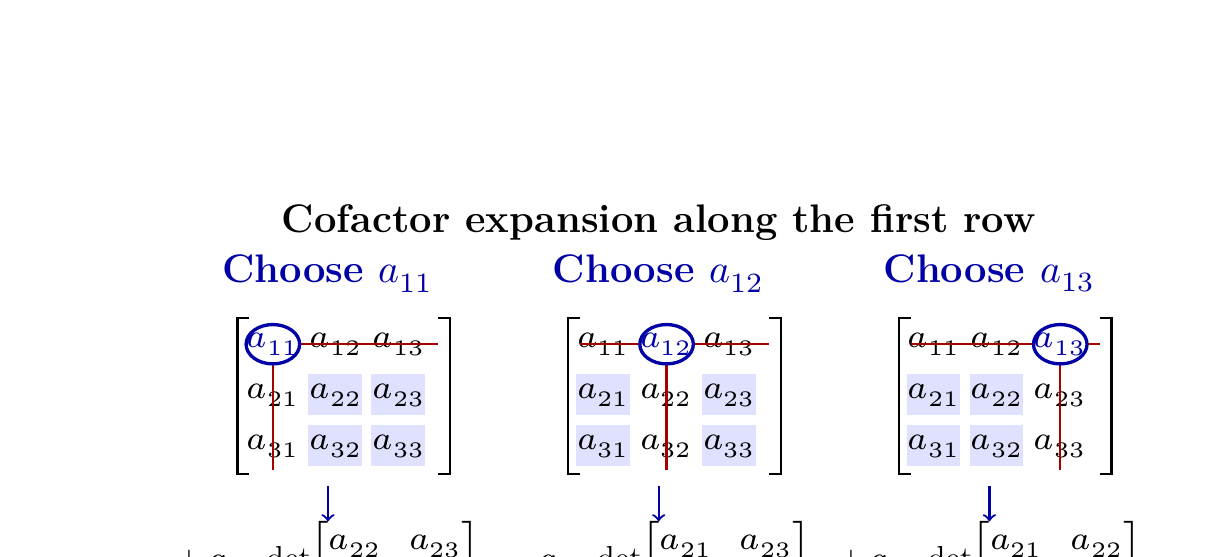
\begin{tikzpicture}[x=1cm,y=1cm,font=\small]
  \node[font=\bfseries] at (6,5.7) {Cofactor expansion along the first row};
  \foreach \j/\cx/\sgn in {1/1.8/+,2/6/-,3/10.2/+} {
    \node[font=\bfseries,text=blue!65!black] at (\cx,5.05) {Choose $a_{1\j}$};
    % The four surviving entries form the minor.
    \foreach \r in {2,3} {
      \foreach \c in {1,2,3} {
        \ifnum\c=\j\relax\else
          \fill[blue!12] (\cx+0.8*\c-1.85,4.55-0.65*\r)
            rectangle ++(0.68,0.52);
        \fi
      }
    }
    \foreach \r in {1,2,3} {
      \foreach \c in {1,2,3} {
        \node at (\cx+0.8*\c-1.5,4.8-0.65*\r) {$a_{\r\c}$};
      }
    }
    \draw[thick] (\cx-1,4.48) -- (\cx-1.15,4.48) -- (\cx-1.15,2.5) -- (\cx-1,2.5);
    \draw[thick] (\cx+1.4,4.48) -- (\cx+1.55,4.48) -- (\cx+1.55,2.5) -- (\cx+1.4,2.5);
    % Cross out row 1 and column j; circle their intersection.
    \draw[red!65!black,thick] (\cx-1,4.15) -- (\cx+1.4,4.15);
    \draw[red!65!black,thick] (\cx+0.8*\j-1.5,4.4) -- (\cx+0.8*\j-1.5,2.55);
    \draw[blue!65!black,very thick,fill=white] (\cx+0.8*\j-1.5,4.15) ellipse (0.34 and 0.25);
    \node[text=blue!65!black] at (\cx+0.8*\j-1.5,4.15) {$a_{1\j}$};
    \draw[->,thick,blue!65!black] (\cx,2.35) -- (\cx,1.9);
  }
  \node at (1.8,1.4) {$+\,a_{11}\det\!\begin{bmatrix}a_{22}&a_{23}\\a_{32}&a_{33}\end{bmatrix}$};
  \node at (6,1.4) {$-\,a_{12}\det\!\begin{bmatrix}a_{21}&a_{23}\\a_{31}&a_{33}\end{bmatrix}$};
  \node at (10.2,1.4) {$+\,a_{13}\det\!\begin{bmatrix}a_{21}&a_{22}\\a_{31}&a_{32}\end{bmatrix}$};
  \node[align=center] at (6,0.35) {Delete the selected entry's row and column. The shaded entries form its minor.\\
    Add the three signed products above to obtain $\det(A)$.};
\end{tikzpicture}
\caption{Expansion of a $3\times3$ determinant along row 1. The signs are $(-1)^{1+j}$: $+$, $-$, $+$.}
\end{figure}


\newpage
%\bigskip

\activity Find the determinant of $$A=\begin{bmatrix} 1 & 2 & 3\\ 4 & 3 & 2 \\ 3 & 2 & 1
\end{bmatrix}$$ by expanding along row 1. Also try expanding along column 2.

\answer[16cm]{Using row 1:
	$\det(A) = 1\cof(A)_{11} + 2\cof(A)_{12} + 3\cof(A)_{13}$
	
	$\cof(A)_{11} = (-1)^{1+1}\det\begin{bmatrix} 3 & 2 \\ 2 & 1 \end{bmatrix} = (1)(3\cdot 1 - 2\cdot 2) = -1$
	
	$\cof(A)_{12} = (-1)^{1+2}\det\begin{bmatrix} 4 & 2 \\ 3 & 1 \end{bmatrix} = (-1)(4\cdot 1 - 2\cdot 3) = 2$
	
	$\cof(A)_{13} = (-1)^{1+3}\det\begin{bmatrix} 4 & 3 \\ 3 & 2 \end{bmatrix} = (1)(8 - 9) = -1$
	
	Therefore: $\det(A) = 1(-1) + 2(2) + 3(-1) = -1 + 4 - 3 = 0$
	
	Using column 2:
	$\det(A) = 2\cof(A)_{12} + 3\cof(A)_{22} + 2\cof(A)_{32}$
	
	$\cof(A)_{12} = (-1)^{1+2}\det\begin{bmatrix} 4 & 2 \\ 3 & 1 \end{bmatrix} = (-1)(4\cdot 1 - 2\cdot 3) = 2$
	
	$\cof(A)_{22} = (-1)^{2+2}\det\begin{bmatrix} 1 & 3 \\ 3 & 1 \end{bmatrix} = (1)(1\cdot 1 - 3\cdot 3) = -8$
	
	$\cof(A)_{32} = (-1)^{3+2}\det\begin{bmatrix} 1 & 3 \\ 4 & 2 \end{bmatrix} = (-1)(2 - 12) = 10$
	
	$\det(A) = 2(2) + 3(-8) + 2(10) = 4 - 24 + 20 = 0$}
	
%\bigskip
\newpage
	
To track the sign $(-1)^{i+j}$, we can view the matrix as a checkerboard pattern:

\answer{$\begin{bmatrix} + & - & + \\ - & + & - \\ + & - & + \end{bmatrix}$}

Note: Since the row/column doesn't matter, you should choose the ``easiest'' row/column:

\bigskip

\activity\label{activity-determinant-zero-row}
$\det\left(\begin{bmatrix} 3 &-5 & 1\\ 0 & 1 & 0 \\ -2 & -4 & 7\end{bmatrix}\right) $

\bigskip

\answer{Using row 2 (has two zeros):
	$\det(A) = 0\cdot\cof(A)_{21} + 1\cdot\cof(A)_{22} + 0\cdot\cof(A)_{23}$
	
	$\cof(A)_{22} = (-1)^{2+2}\det\begin{bmatrix} 3 & 1\\ -2 & 7\end{bmatrix}$
	$= (1)(3\cdot 7 - 1\cdot(-2))$
	$= 21 + 2 = 23$.
	Therefore $\det(A) = 23$
	}

\bigskip

$\det\left(\begin{bmatrix} 0 & \pi & 200\\ 0 & 0.03 & 4 \\ 0 & 19 & -3584\end{bmatrix}\right) $

\bigskip

\answer{Using column 1 (all zeros):
	$\det(A) = 0\cdot\cof(A)_{11} + 0\cdot\cof(A)_{21} + 0\cdot\cof(A)_{31} = 0$
	
	Note: When a row or column is all zeros, the determinant is automatically 0. We didn't need to calculate the cofactors.}
	
	
%\bigskip
\newpage

We can compute the determinant of a general $n\times n$ matrix by recursively repeating this process:

\activity 
$A=\begin{bmatrix} 1 & 2 & 3 & 4 \\ 5 & 4 & 2 & 3\\ 1 & 3 & 4 & 5 \\ 3 & 4 & 3 & 2\end{bmatrix}$, if we expand along third column, we get
 
\bigskip
 
 \answer[12cm]{
\begin{align*}
	&\det(A)=3(-1)^{1+3}\det\left(\begin{bmatrix} 5 & 4 & 3 \\ 1 & 3 & 5\\ 3 & 4 & 2\end{bmatrix}\right)\\
	&+2(-1)^{2+3}\det\left(\begin{bmatrix} 1 & 2 & 4\\ 1 & 3 & 5\\ 3 & 4 & 2\end{bmatrix}\right)\\
	&+4(-1)^{3+3}\det\left(\begin{bmatrix} 1 & 2 & 4\\ 5 &4 & 3\\ 3 & 4 & 2\end{bmatrix}\right)\\
	&+3(-1)^{4+3}\det\left(\begin{bmatrix} 1 & 2 & 4\\ 5 & 4 & 3\\ 1 & 3 & 5\end{bmatrix}\right)=-12.
\end{align*}
}


\bigskip

\definition  Let $A$ be a $n\times n$ matrix ($n\geq 3)$. Then the \fillin{determinant} of $A$, $\det(A)$, is

$$\det(A)=\sum_{j=1}^n a_{ij}\cof(A)_{ij}=\sum_{i=1}^n a_{ij}\cof(A)_{ij}$$

for some choice of row $i$ or column $j$.

%\bigskip
\newpage

\activity\label{activity-triangular-determinant} Compute $\det(A)$ for $A = \begin{bmatrix} 3 & 2 & 3 & 4 \\ 0 & 4 & 2 & 3\\ 0 & 0 & 2 & 5 \\ 0 & 0 & 0 & -1\end{bmatrix}$

\bigskip

\answer[10cm]{Using column 1 (3 zeros):
	$\det(A) = 3\cdot\cof(A)_{11} + 0\cdot\cof(A)_{21} + 0\cdot\cof(A)_{31} + 0\cdot\cof(A)_{41}$
	$= 3\cdot\cof(A)_{11}$
	$= 3\cdot(-1)^{1+1}\det\begin{bmatrix} 4 & 2 & 3\\ 0 & 2 & 5\\ 0 & 0 & -1\end{bmatrix}$
	
	Looking at this $3\times 3$ determinant, use column 1 again:
	$= 3\cdot(1)\cdot[4\cdot\det\begin{bmatrix} 2 & 5\\ 0 & -1\end{bmatrix}]$
	$= 3\cdot 4\cdot[2\cdot(-1) - 5\cdot 0]$
	$= 3\cdot 4\cdot(-2)$
	$= -24$
	
	Alternative justification: Since $A$ is upper triangular, $\det(A)$ is the product of diagonal entries:
	$\det(A) = 3\cdot 4\cdot 2\cdot(-1) = -24$}
	
\bigskip

\definition The \fillin{main diagonal} of an $\nbyn$ matrix $A$ is the set of entries $(a_{11}, a_{22}, \ldots , a_{nn})$.

\bigskip

\definition An $\nbyn$ matrix $A = [\aij]$ is called \fillin{upper triangular} if \fillin{$a_{ij} = 0$} for $i>j$, and $A$ is called \fillin{lower triangular} if \fillin{$a_{ij} = 0$} for $i < j$.\\ A \fillin{diagonal matrix} is both upper and lower triangular.

\bigskip

\theorem If $A=[a_{ij}]$ is a upper/lower triangular matrix, then $\det(A)=a_{11}a_{22}\cdots a_{nn}$, that is, the determinant of a triangular matrix is the product of the elements on the \fillin{main diagonal}.

%\textit{Justification chat: (i.e. ``proof''):}

\answer[1cm]{See Activity~\ref{activity-triangular-determinant}.}

%\bigskip
\newpage

\topic{Properties of Determinants} 

\bigskip

\theorem If a row (column) of $A$ consists entirely of zeros, then $\det(A)=0$.

\proof

\answer[1cm]{See Activity~\ref{activity-determinant-zero-row}.}

\theorem If $B$ results from $A$ by interchanging two different rows (or two different columns), then $\det(B)=-\det(A)$.

\proof

\answer{Check for $2 \times 2$: $A=\begin{bmatrix}a & b \\ c & d \end{bmatrix}$ and $\det(A)=ad-bc.$ OTOH, $B=\begin{bmatrix}c & d \\ a & b \end{bmatrix}$ and $\det(B)= cb - ad = -(ad-bc).$ 
}

\bigskip

\theorem If two rows (columns) of $A$ are equal,then $\det(A)=0$.

\proof

\answer{Let $B$ be the matrix obtained by interchanging these two equal rows. Then $B=A$ (since the rows were equal) but also $\det(B)=-\det(A)$ (by the previous theorem about row interchanges). Therefore:
	$\det(A) = \det(B) = -\det(A)$.
	This implies $2\det(A) = 0$, so $\det(A) = 0$.}



\theorem If $B$ is obtained from $A$ by multiplying a row (column) of $A$ by a real number $k$, then $\det(B)=k\det(A)$.

\proof

\answer[5cm]{Suppose row $i$ is multiplied by $k$. Expand along that row
\begin{align*}
	&\det(k A)=k a_{i1}\cof(kA)_{i1}+ k a_{i2}\cof(kA)_{i2}+k a_{i3}\cof(kA)_{i3}\\
	& =k a_{i1}\cof(A)_{i1}+ k a_{i2}\cof(A)_{i2}+k a_{i3}\cof(A)_{i3} = k \det(A)\end{align*}
	since $\cof(kA)_{ij}$ does not depend on the $i$-th row.
}


\fact If $A$ is an $n\times n$ matrix, then $\det(k A)=$\fillin{$k^n \det(A)$}.

\bigskip

\theorem If $B$ is obtained by adding $k$ times the $i$th row of $A$ to the $j$th row ($i\neq j$), written as $R_j \to R_j + k R_i$, then $\det(A)=\det(B)$.

Check for $2\times 2$:
$\det\left(\begin{bmatrix}a & b \\ c & d \end{bmatrix}\right) = $\shortanswer{$ad-bc$}

$\det\left(\begin{bmatrix}a & b \\ ka+c & kb+d \end{bmatrix}\right) =$ 

\bigskip

\answer[1cm]{$a(kb+d)-b(ka+c) = akb + ad - bka - bc = ad-bc$}

\begin{framed}\textbf{Row Operations and the Determinant:}
	Here is a summary of how the elementary row operations affect the determinant:
	\begin{enumerate}
		\item Type I (scaling): $R_i \to kR_i$ multiplies determinant by $k$
		\item Type II (interchange): $R_i \leftrightarrow R_j$ multiplies determinant by $-1$
		\item Type III (replacement): $R_j \to R_j + kR_i$ leaves determinant unchanged
	\end{enumerate}
\end{framed}

\activity If $B$ is obtained from $A$ by the following operations: $R_1 \leftrightarrow R_2$, $R_4 \to 4R_4$, and $R_3 \to R_3 + 3R_2$, and $\det(A)=8$, what is the determinant of $B$?

\answer{
	$R_1 \leftrightarrow R_2$: multiplies det by $-1$
	
	$R_4 \to 4R_4$: multiplies det by $4$  
	
	$R_3 \to R_3 + 3R_2$: no change in det
	
	Therefore $\det(B) = -1 \cdot 4 \cdot 1 \cdot \det(A) = -32$}

\newpage

\activity Compute the determinant of the matrix
$
B = \barray{rrr}{1 & 2 & 1 \\ -1 & 3 & 3 \\ 0 & 15 & 12}$

\bigskip

\answer[10cm]{Use row operations to make the matrix upper triangular:
	
	$B = \begin{bmatrix} 1 & 2 & 1\\ -1 & 3 & 3\\ 0 & 15 & 12\end{bmatrix}$
	
	$R_2 \to R_2 + R_1$:
	$\begin{bmatrix} 1 & 2 & 1\\ 0 & 5 & 4\\ 0 & 15 & 12\end{bmatrix}$
	
	$R_3 \to R_3 - 3R_2$:
	$\begin{bmatrix} 1 & 2 & 1\\ 0 & 5 & 4\\ 0 & 0 & 0\end{bmatrix}$
	
	Now we have an upper triangular matrix. The determinant is $0$ because we have a row of zeros.}
	

\newpage



\sectiontitle{3.2}{Determinants and Matrix Inverses} 



\theorem If $A$ and $B$ are $\nbyn$ matrices, then $\det(AB)=$\fillin{$\det(A) \det(B)$}. 

\activity Compute the determinant of $A$, $B$, $C$, $AC$, and $BC$, where $A$, $B$, and $C$ are the matrices 
\[
A = \twobytwo{3}{1}{-2}{7},
\: 
B = \twobytwo{1}{2}{2}{4},
\text{ and } 
C = \twobytwo{1}{4}{0}{2}.
\] 
Confirm (if time) that $\det(AC) = \det(A)\det(C)$ and $\det(BC) = \det(B)\det(C)$. 

\bigskip

\answer[9cm]{
	For $A$: $\det(A) = 3(7) - 1(-2) = 23$
	
	For $B$: $\det(B) = 1(4) - 2(2) = 0$
	
	For $C$: $\det(C) = 1(2) - 4(0) = 2$
	
	For $AC$:
	$AC = \begin{bmatrix} 3 & 1\\ -2 & 7\end{bmatrix}\begin{bmatrix} 1 & 4\\ 0 & 2\end{bmatrix} = \begin{bmatrix} 3 & 14\\ -2 & 6\end{bmatrix}$, 
	$\det(AC) = 3(6) - 14(-2) = 18 + 28 = 46$.
	And indeed $\det(A)\det(C) = 23 \cdot 2 = 46$
	
	For $BC$:
	$BC = \begin{bmatrix} 1 & 2\\ 2 & 4\end{bmatrix}\begin{bmatrix} 1 & 4\\ 0 & 2\end{bmatrix} = \begin{bmatrix} 1 & 8\\ 2 & 16\end{bmatrix}$, 
	$\det(BC) = 1(16) - 8(2) = 0$. 
	And indeed $\det(B)\det(C) = 0 \cdot 2 = 0$.
}

\theorem If $A$ is an $\nbyn$ matrix, then $A$ is \fillin{nonsingular} if and only if $\det(A)$\fillin{$\ne 0$}. In this case, $\det(A^{-1})=\dfrac{1}{\det(A)}$.

\emph{Proof:}

\answer{($\Rightarrow$) Assume $A$ is nonsingular. Then $AA^{-1} = I$. Taking determinants of both sides:
	$\det(AA^{-1}) = \det(I)$ so simplifying
	$\det(A)\det(A^{-1}) = 1$. 
	Therefore $\det(A) \neq 0$ and $\det(A^{-1}) = \frac{1}{\det(A)}$.}


%\bigskip
\newpage

\theorem If $A$ is a square matrix, then $\det(A)=\det(A^T)$.

\activity Let $A$ be a square matrix. A matrix is called orthogonal if $A^{-1} = A^T$. What are the possible values of $\det A$ if $A$ is orthogonal?

\answer[5cm]{If $A$ is orthogonal, we have $I = AA^T$. Taking determinants of both sides:
	
	$1 = \det(I) = \det(AA^T) = \det(A)\det(A^T) = \det(A)\det(A) = (\det A)^2$
	
	Therefore, $\det A = \pm 1$.}

\end{document}

